\section{Price response function definitions}
\label{sec:response_functions_def}

In Sect. \ref{subsec:key_concepts} we introduce the fundamental quantities used
in the price response definitions. In Sect. \ref{subsec:time_definition} we
describe the physical time scale and the trade time scale. We introduce the
price response functions used in literature in Sect. \ref{subsec:response_def}.

%%%%%%%%%%%%%%%%%%%%%%%%%%%%%%%%%%%%%%%%%%%%%%%%%%%%%%%%%%%%%%%%%%%%%%%%%%%%%%%
\subsection{Key concepts}\label{subsec:key_concepts}

Market orders are execute at the best available buy or sell price, limit orders
set a maximum purchase price for a buy order, or a minimum sale price for a
sell order. If the limit price is not matched, the order will not be carried
out
\cite{large_prices_changes,predictive_pow,intro_market_micro,stat_theory}.
Limit orders often fail to result in an immediate transaction, and are stored
in a queue called the limit order book
\cite{prop_order_book,stat_prop,predictive_pow,intro_market_micro}. The order
book also identifies the market participants behind the buy and sell orders,
although some choose to remain anonymous. The order book is visible for all
traders and its main purpose is to ensure that all traders have the same
information on what is offered on the market. The order book is the ultimate
microscopic level of description of financial markets.

Buy limit orders are called ``bids", and sell limit orders are called ``asks".
At any given time there is a best (lowest) offer to sell with price
$a\left(t\right)$, and a best (highest) bid to buy with price $b\left(t\right)$
\cite{prop_order_book,subtle_nature,account_spread,limit_ord_spread,stat_theory}.
The price gap between them is called the spread
$s\left(t\right) = a\left(t\right)-b\left(t\right)$
\cite{subtle_nature,market_digest,Bouchaud_2004,account_spread,large_prices_changes,em_stylized_facts,stat_theory}.
Spreads are significantly positively related to price and significantly
negatively related to trading volume. Companies with more liquidity tend to
have lower spreads
\cite{components_spread_tokyo,effects_spread,account_spread,components_spread}.

The average of the best ask and the best bid is the midpoint price, which is
defined as
\cite{prop_order_book,subtle_nature,Bouchaud_2004,large_prices_changes,em_stylized_facts,stat_theory}
\begin{equation}\label{eq:midpoint_price}
    m\left(t\right)=\frac{a\left(t\right)+b\left(t\right)}{2}
\end{equation}
As the midpoint price depends on the quotes, it changes if the quotes change.
The midpoint price grows if the best ask or the best bid grow. On the other
hand, the midpoint price decreases if the best ask or the best bid
decrease.

Price changes are typically characterized as returns. If one denotes
$S\left( t\right)$ the price of an asset at time $t$, the return
$r^{\left(g\right)}\left(t, \tau\right)$, at time $t$ and time lag $\tau$ is
simply the relative variation of the price from $t$ to $t + \tau$
\cite{subtle_nature,empirical_facts,asynchrony_effects_corr,tick_size_impact,causes_epps_effect,non_stationarity},
\begin{equation}\label{eq:return_general}
    r^{\left(g\right)} \left(t, \tau \right) = \frac{S\left(t + \tau\right)
    - S\left(t\right)}{S\left(t\right)}
\end{equation}
It is also common to define the returns as
\cite{dissecting_cross,subtle_nature,empirical_facts,empirical_properties,large_prices_changes,pow_law_dist,theory_market_impact,spread_changes_affect,rand_mat,fluctions_market_friction}
\begin{equation}\label{eq:log_return_general}
    r^{\left(l\right)}\left(t,\tau\right) = \ln S\left(t + \tau\right)
    - \ln S\left(t\right) = \ln \frac{S\left(t + \tau\right)}{S\left(t\right)}
\end{equation}
Equations (\ref{eq:return_general}) and (\ref{eq:log_return_general}) agree if
$\tau$ is small enough \cite{subtle_nature,empirical_facts}.

At longer timescales, midpoint prices and transaction prices rarely differ by
more than half the spread. The midpoint price is more convenient to study
because it avoids problems associated with the tendency of transaction prices
to bounce back and forth between the best bid and ask
\cite{large_prices_changes}.

We define the returns via the midpoint price as
\begin{equation}\label{eq:midpoint_price_return}
    r\left(t,\tau\right) = \frac{m\left(t+\tau\right)-m\left(t\right)}
    {m\left(t\right)}
\end{equation}
The distribution of returns is strongly non-Gaussian and its shape continuously
depends on the return period $\tau$. Small $\tau$ values have fat tails return
distributions \cite{subtle_nature}. The trade signs are defined for general
cases as
\begin{equation}\label{eq:trade_sign_general}
    \varepsilon\left(t\right)=\text{sign}\left(S\left(t\right)
    -m\left(t-\delta\right)\right)
\end{equation}
where $\delta$ is a positive time increment. Hence we have
\begin{equation}\label{eq:trade_sign_results}
    \varepsilon\left(t\right)=\left\{
    \begin{array}{cc}
    +1, & \text{If } S\left(t\right)
    \text{ is higher than the last } m\left( t \right)\\
    -1, & \text{If } S\left(t\right)
    \text{ is lower than the last } m\left( t \right)
    \end{array}\right.
\end{equation}
$\varepsilon(t) = +1$ indicates that the trade was triggered by a market order
to buy and a trade triggered by a market order to sell yields
$\varepsilon(t) = -1$
\cite{subtle_nature,Bouchaud_2004,spread_changes_affect,quant_stock_price_response,order_flow_persistent}.

It is well-known that the series of the trade signs on a given stock exhibit
large autocorrelation. A very plausible explanation of this phenomenon relies
on the execution strategies of some major brokers on given markets. These
brokers have large transactions to execute on the account of some clients. In
order to avoid market making movements because of an inconsiderable large
order, they tend to split large orders into small ones \cite{empirical_facts}.

%%%%%%%%%%%%%%%%%%%%%%%%%%%%%%%%%%%%%%%%%%%%%%%%%%%%%%%%%%%%%%%%%%%%%%%%%%%%%%%
\subsection{Time definition}\label{subsec:time_definition}

A direct comparison between the trade time scale and the physical time scale is
not possible. To compare them directly we need to assume whether the midpoint
price or the trade signs are on the same scale. We assume the midpoint prices
in the trade time scale to be the same as the midpoint prices in physical time
scale. Therefore, we have the time lag for both computations in seconds. This
approximation allow us to directly compare both scales to have an idea of the
difference and similarities they have. In the other sections, as we are not
directly comparing the time scales, the corresponding quantities of each time
scale are not mixed. Thus physical time scale is measured in seconds and trade
time scale is measured in trades.

Due to the nature of the data, they are several options to define time for
analyzing data.

In general, the time series are indexed in calendar time (hours, minutes,
seconds, milliseconds). Moreover, tick-by-tick data available on financial
markets all over the world is time stamped up to the millisecond, but the order
of magnitude of the guaranteed precision is much larger, usually one second or
a few hundreds of milliseconds \cite{market_digest,empirical_facts}. In several
papers are used different time definitions (calendar time, physical time, event
time, trade time, tick time)
\cite{empirical_facts,sampling_returns,market_making}. The TAQ data used in the
analysis has the characteristic that the trades and quotes can not be directly
related due to the time stamp resolution of only one second
\cite{Wang_2016_cross}. Hence, it is impossible to match each trade with the
directly preceding quote. However, using a classification for the trade signs,
we can compute trade signs in two scales: trade time scale and physical time
scale.

The trade time scale is increased by one unit each time a transaction happens.
The advantage of this count is that limit orders far away in the order book do
not increase the time by one unit. The main outcome of trade time scale is its
``smoothing" of data and the aggregational normality \cite{empirical_facts}.

The physical time scale is increased by one unit each time a second passes.
This means that computing the responses in this scale involves sampling
\cite{sampling_returns,Wang_2016_cross}, which has to be done carefully when
dealing for example with several stocks with different liquidity. This sampling
is made in the trade signs and in the midpoint prices.

Facing the impossibility to relate midpoint prices and trade signs with the TAQ
data in trade time scale, we will use the midpoint price of the previous second
with all the trade signs of the current second. This will be our definition of
trade time scale analysis for the response function analysis.

For physical time scale, as we can sampling, we relate the unique value of
midpoint price of a previous second with the unique trade sign value of the
current second.

%%%%%%%%%%%%%%%%%%%%%%%%%%%%%%%%%%%%%%%%%%%%%%%%%%%%%%%%%%%%%%%%%%%%%%%%%%%%%%%
\subsubsection*{Trade time scale}\label{subsubsec:trade_time}

We use the trade sign classification in trade time scale proposed in Ref.
\cite{Wang_2016_cross} and used in Refs.
\cite{Wang_2017,Wang_2018_copulas,Wang_2016_avg} that reads

\begin{equation}\label{eq:trade_signs_trade}
    \varepsilon^{\left(t\right)}\left(t,n\right)=\left\{
    \begin{array}{cc}
    \text{sgn}\left(S\left(t,n\right)-S\left(t,n-1\right)\right),
    & \text{if }\\ S\left(t,n\right) \ne S\left(t,n-1\right)\\
    \varepsilon^{\left(t\right)}\left(t,n-1\right),
    & \text{otherwise}
    \end{array}\right.
\end{equation}

$\varepsilon^{\left(t\right)}\left( t,n \right) = +1$ implies a trade triggered
by a market order to buy, and a value
$\varepsilon^{\left(t\right)}\left( t,n \right) = -1$ indicates a trade
triggered by a market order to sell.

In the second case of Eq. (\ref{eq:trade_signs_trade}), if two consecutive
trades with the same trading direction did not exhaust all the available volume
at the best quote, the trades would have the same price, and in consequence
they will have the same trade sign.

With this classification we obtain trade signs for every single trade in the
data set. According to Ref. \cite{Wang_2016_cross}, the average accuracy of the
classification is $85\%$ for the trade time scale.

The TAQ time step is one second, and as it is impossible to find the
correspondences between trades and midpoint prices values inside a second step,
We used the last midpoint price of every second as the representative value of
each second. This introduce an apparent shift between trade signs and returns.
In fact, we set the last midpoint price from the previous second as the first
midpoint price of the current second \cite{Wang_2016_cross}.

As we know the second in which the trades were made, we can relate the trade
signs and the midpoint prices as shown in Fig.
\ref{fig:relation_trades_midpoint_trade_scale}. For the trade time scale, there
are in general, several midpoint prices in a second. For each second we select
the last midpoint price value, and we relate it to the next second trades. In
Fig. \ref{fig:relation_trades_midpoint_trade_scale}, the last midpoint price
(circle) between the second $-1$ and $0$ is related to all the trades (squares
and triangles) in the second $0$ to $1$, and so on. In the seconds when the
quotes do not change, the value of the previous second (vertical line over the
physical time interval) is used. Thus, all the seconds in the open market time
have a midpoint price value, and in consequence returns values. We assume that
as long as no changes ocurred in the quotes, the midpoint price remains the
same as in the previous second.

\begin{figure}[htbp]
    \centering
    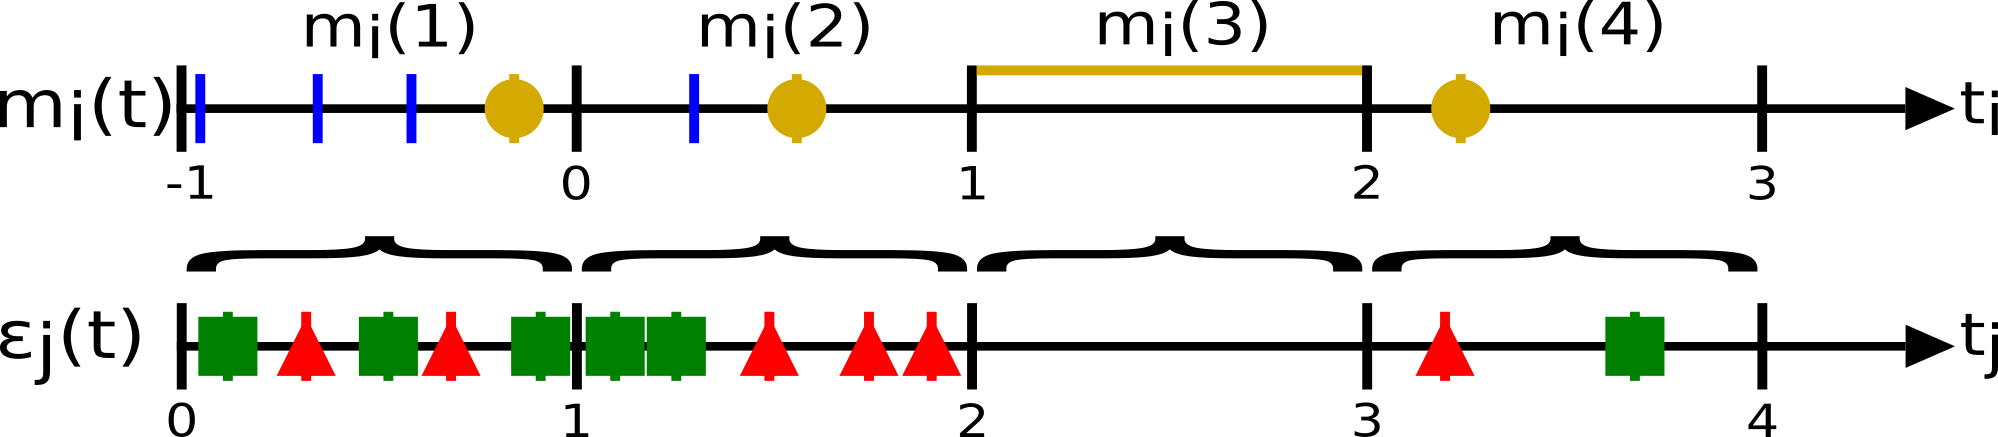
\includegraphics[width=\columnwidth]
    {figures/02_relation_trades_quotes_trade_scale.png}
    \caption{Sketch of data processing for trade time scale. In the midpoint
             price time line, the vertical lines represent the change in price
             of the quotes and the circles represent the last price change in a
             quote in a second. In the trade signs time line, the squares
             represent the buy market orders and the triangles represent the
             sell market orders. The midpoint price time line and the trade
             sign time line are shifted in one second.}
    \label{fig:relation_trades_midpoint_trade_scale}
\end{figure}

The methodology described is an approximation to compute the response in the
trade time scale. A drawback in the computation could come from the fact that
the return of a given second is composed by the contribution of small returns
corresponding to each change in the midpoint price during a second. As we are
assuming only one value for the returns in each second, we consider all the
returns in one second interval to be positive or negative with the same
magnitude, which could not be the case. This could increase or decrease the
response signal at the end of the computation.

\begin{figure}[htbp]
    \centering
    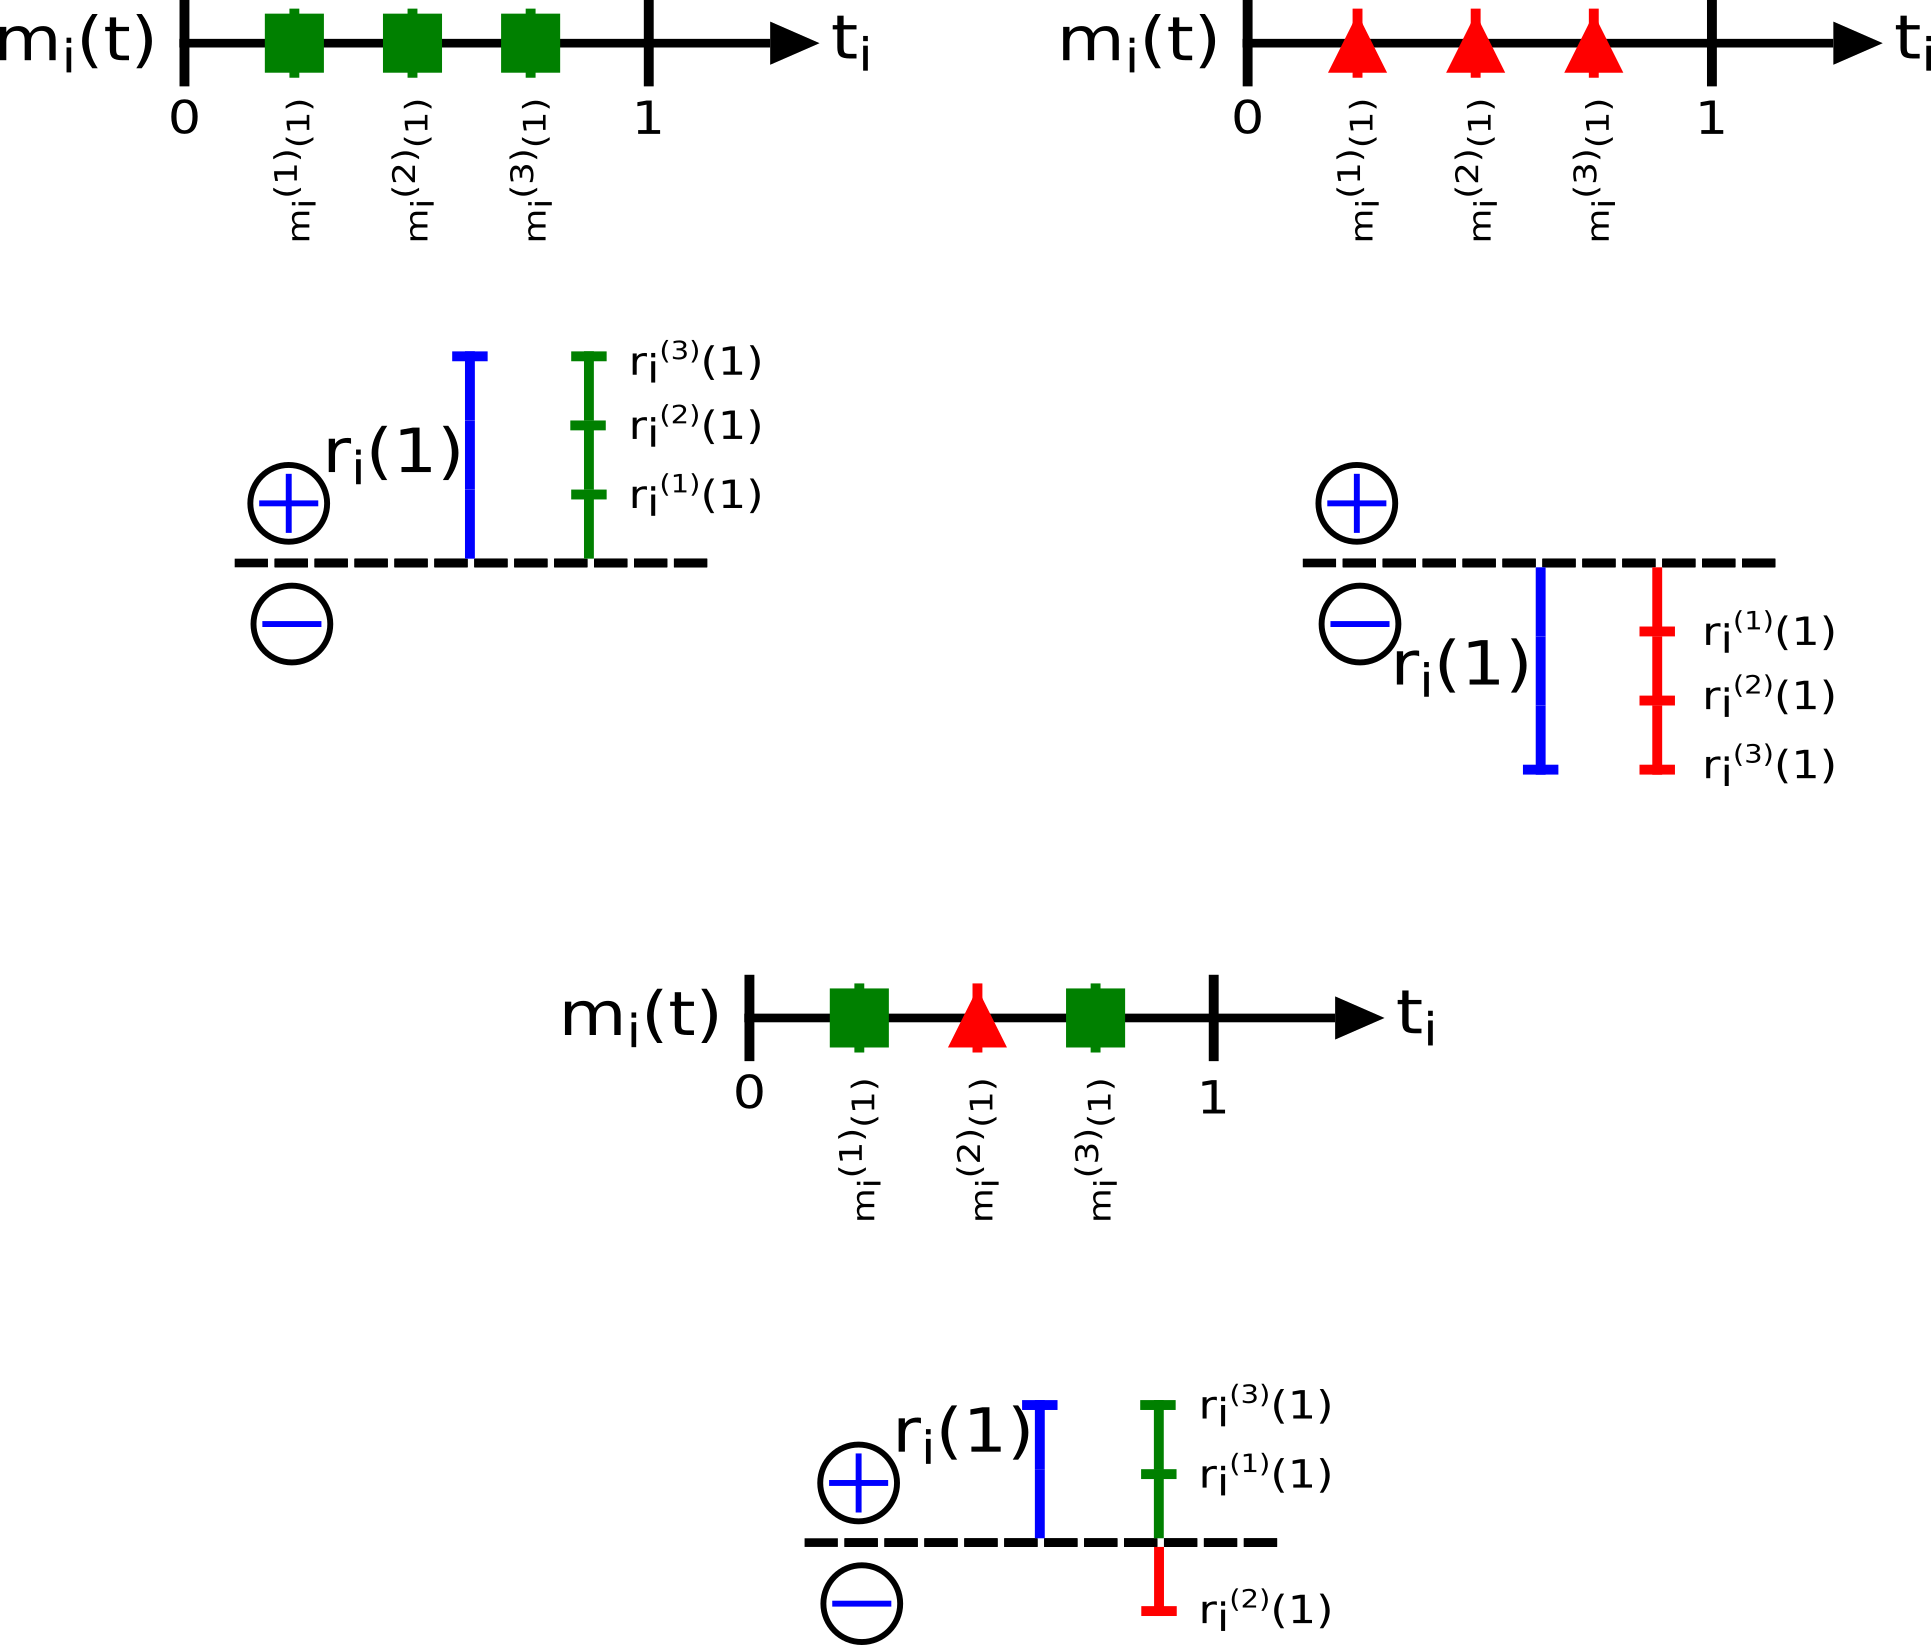
\includegraphics[width=\columnwidth]{figures/02_return_contributions.png}
    \caption{Sketch of the return contributions from every midpoint price
             change in a second. The squares represent the rise of the price of
             the midpoint price and the triangles represent the decrease of the
             price of the midpoint price. We illustrate three cases: (top left)
             the changes of the midpoint prices and return are due to the rise
             of the prices, (top right) the changes of the midpoint prices and
             return are due to the decrease of the prices, and (bottom) the
             changes of the midpoint prices and return are due to a combination
             of rise and decrease of the prices. The blue vertical line
             represents the net return in each case.}
    \label{fig:return_contributions}
\end{figure}

Figure \ref{fig:return_contributions} illustrate this point. Suppose there are
three different midpoint prices in one second interval and thus, three
different returns for these three midpoint price values. Furthermore, suppose
that the volume of limit orders with the corresponding midpoint prices are the
same in the bid and in the ask (the returns have the same magnitude). In the
case of the top left (top right) sketch, all the changes are due to the rise
(decrease) of the midpoint price, that means, consumption of the best ask
(bid), so all the contributions of the individual returns in the second are
positive (negative), and in consequence, the net return is positive (negative).
In the case of the bottom, the changes are due to a combination of increase and
decrease of the midpoint price, so in the end, the individual returns sum up to
a net return, which can be positive or negative, depending of the type of
midpoint price values in the interval. Thus, in this case, we are assuming in
the end that all the returns were positive or negative, which probably was not
the case, and in consequence will increase or decrease the real value of the
net return.

In all cases, we choose the last change in the midpoint price in a second
interval as described before in Fig.
\ref{fig:relation_trades_midpoint_trade_scale}. We use this method knowing that
the variation in one second of the midpoint price is not large (in average, the
last midpoint price of a second differ with the average midpoint of that second
in $0.007\%$), hence it can give us representative information on the response
functions.

%%%%%%%%%%%%%%%%%%%%%%%%%%%%%%%%%%%%%%%%%%%%%%%%%%%%%%%%%%%%%%%%%%%%%%%%%%%%%%%
\subsubsection*{Physical time scale}\label{subsubsec:physical_time}

We use the trade sign definition in physical time scale proposed in Ref.
\cite{Wang_2016_cross} and used in Refs.
\cite{Wang_2017,Wang_2016_avg}, that depends on the classification in
Eq. (\ref{eq:trade_signs_trade}) and reads
\begin{equation}\label{eq:trade_signs_physical}
    \varepsilon^{\left(p\right)}\left(t\right)=\left\{
    \begin{array}{cc}
    \text{sgn}\left(\sum_{n=1}^{N\left(t\right)}\varepsilon^{\left(t\right)}
    \left(t,n\right)\right),
    & \text{If }N \left(t\right)>0\\
    0, & \text{If }N\left(t\right)=0
    \end{array}\right.
\end{equation}
where $N \left(t \right)$ is the number of trades in a second interval.
$\varepsilon^{\left(p\right)}\left( t \right) = +1$ implies that the majority
of trades in second $t$ were triggered by a market order to buy, and a value
$\varepsilon^{\left(p\right)}\left( t \right) = -1$ indicates a majority of
sell market orders. In this definition, they are two ways to obtain
$\varepsilon^{\left(p\right)}\left( t \right) = 0$. One way is that in a
particular second there are no trades, and then no trade sign. The other way is
that the addition of the trade signs ($+1$ and $-1$) in a second be equal to
zero. In this case, there is a balance of buy and sell market orders.

Market orders show opposite trade directions to limit order executed
simultaneously. An executed sell limit order corresponds to a buyer-initiated
market order. An executed buy limit order corresponds to a seller-initiated
market order.

As the trade time scale, on the physical time scale we use the same strategy
to obtain the midpoint price for every second, so all the seconds in the open
market time have a midpoint price value. Even if there is no change of quotes
in a second, it still has a midpoint price value and return value.

\begin{figure}[htbp]
    \centering
    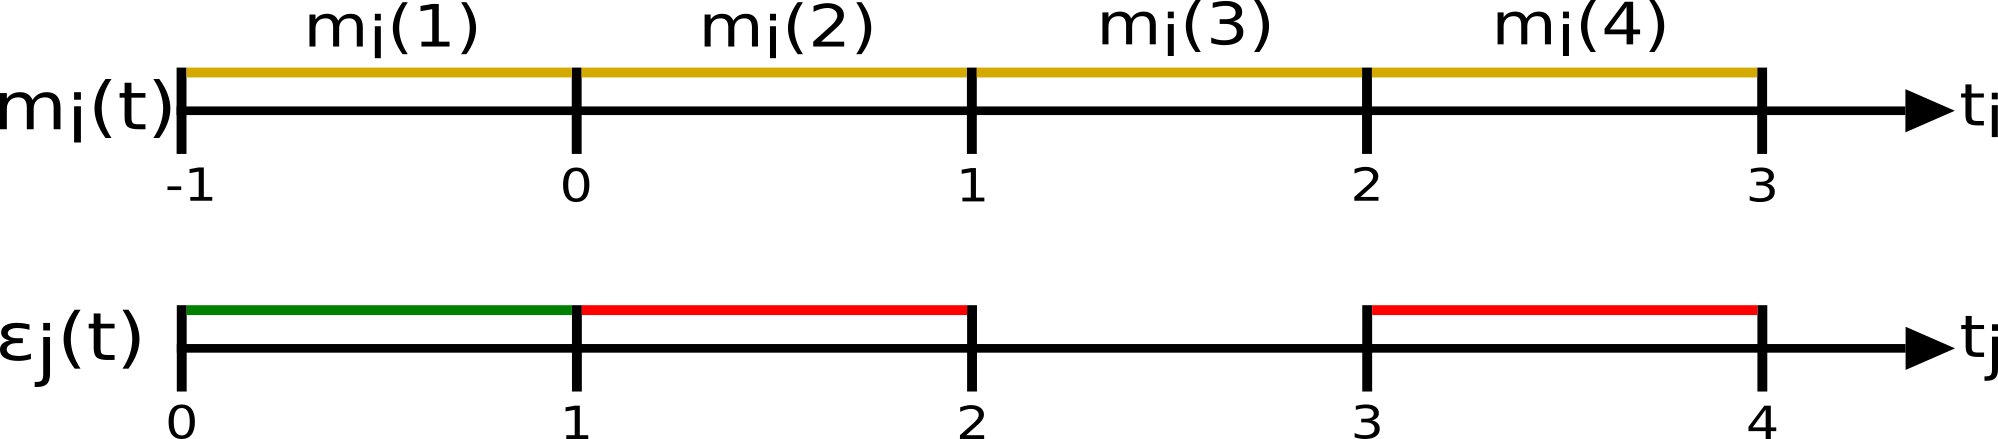
\includegraphics[width=\columnwidth]
    {figures/02_relation_trades_quotes_time_scale.png}
    \caption{Sketch of data processing for physical time scale. In the midpoint
             price time line, the horizontal lines between seconds represent
             the midpoint prices. In the trade signs time line, the horizontal
             lines between seconds represent the trade sign values. The
             midpoint price time line and the trade sign time line are shifted
             in one second.}
    \label{fig:relation_trades_midpoint_time_scale}
\end{figure}

In this case we do not compare every single trade sign in a second, but the net
trade sign obtained for every second with the definition, see
Eq. (\ref{eq:trade_signs_physical}). This can be seen in
Fig. \ref{fig:relation_trades_midpoint_time_scale}, where we related the
midpoint price of the previous second with the trade sign of the current
second. According to Ref. \cite{Wang_2016_cross}, this definition has an
average accuracy up to $82\%$ in the physical time scale.

%%%%%%%%%%%%%%%%%%%%%%%%%%%%%%%%%%%%%%%%%%%%%%%%%%%%%%%%%%%%%%%%%%%%%%%%%%%%%%%

\subsection{Response function definitions}\label{subsec:response_def}

The response function measures price changes resulting from execution of market
orders. In Refs.
\cite{r_walks_liquidity,subtle_nature,Bouchaud_2004}, Bouchaud et al. use a
self-response function that only depends on the time lag $\tau$. This function
measures how much, on average, the price moves up (down) at time $\tau$
conditioned to a buy (sell) order at time zero. They found for France Telecom
that the response function increases by a factor $~2$ between $\tau = 1$ and
$\tau \approx 1000$ trades, before decreasing back. For larger $\tau$, the
response function decreases, and even becomes negative beyond
$\tau \approx 5000$. However, in some cases the maximum is not observed and
rather the price response function keeps increasing mildly
\cite{subtle_nature}.

In Ref. \cite{theory_market_impact}, the price impact function, is defined as
the average price response due to a transaction as a function of the
transaction's volume. Empirically the function is highly concave
\cite{theory_market_impact}. The curvature of the price impact function is
entirely due to the probability that a transaction causes a nonzero impact. The
larger the size of the transaction, the larger the probability. In Ref.
\cite{prop_order_book}, they found that the response function for three French
stocks first increases from $\tau = 10s$ to a few hundred seconds, and then
appears to decrease back to a finite value.

In Ref. \cite{dissecting_cross} they defined a response function who measures
the average price change of a contract $i$ at time $t+\tau$, after experiencing
a sign imbalance in contract $j$ at time $t$. In this work $\tau$ is used in
units of five minutes.

In later works \cite{spread_changes_affect,Wang_2016_cross}, Grimm et al.
and Wang et al. use the logarithmic return for stock $i$ and time lag $\tau$,
defined via the midpoint price $m_{i} \left( t \right)$ to define a
cross-response function. The response function measures how a buy or sell order
at time $t$ influences on average the price at a later time $t + \tau$.
The physical time scale was chosen since the trades in different stocks are not
synchronous (TAQ data). They found that in all cases, an increase  to a
maximum is followed by a decrease. The trend is eventually reversed.

Finally, in Ref. \cite{Wang_2018_b}, Wang et al. define the response function
on a trade time scale (Totalview data), as the interest is to analyze the
immediate responses. Here, the time lag $\tau$ is restricted to one trade, such
that the price response quantifies the price impact of a single trade.
